% !TEX root =/Users/martabellesmunoz/Dropbox/Documents/Especificacions/Merkle trees/Description.tex


Dibuixet + explicacions\\

\begin{center}
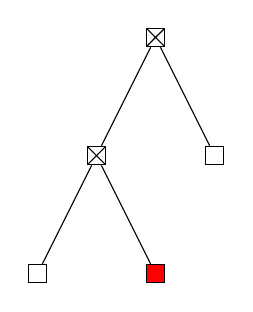
\begin{tikzpicture}[auto,node distance=1.5cm]
	\tikzstyle{internal}  = [draw, path picture={\draw (path picture bounding box.south east) -- (path picture bounding box.north west) (path picture bounding box.south west) -- (path picture bounding box.north east);}]
	\tikzstyle{leaf} = [draw, fill]
	 \tikzstyle{empty} = [draw]
	 \tikzstyle{wrong} = [draw, fill = red]
	 
\node [internal] (r){ }
  child { node [internal]  (a) { }
    		child {node [empty] (c) { }}
    		child {node [wrong] (d) { }}
  	}
  child { node [empty] (b) { } };
\end{tikzpicture}
\end{center}

